\documentclass[a4paper, 10pt]{article}
\usepackage[sorting=none]{biblatex}
\usepackage{graphicx}

\title{Research Progress Report}
\author{Michael Rawson\\3-year PhD, year 1\\ORCID: 0000--0001--7834--1567}
\date{June 2018}
\addbibresource{report-references.bib}
\begin{document}
\maketitle
\section{Background}
I research the application of machine learning techniques to automated theorem provers for first-order logic.

\subsection{Introduction}
Automated provers belong to the field of automated reasoning (see \cite{survey} for an overview), which broadly aims to automate various kinds of reasoning, such as proof (in various logics)~\cite{LEO, Satallax, Isabelle, E, iProver, Vampire, CVC4, Spass, Z3}, disproof by counter-example~\cite{Nitpick, Refute, MACE}, invariant generation~\cite{invariant}, or even abduction~\cite{science-abduction, abduction}.
Theorem provers have many possible applications, such as formal verification of both mathematics and software~\cite{survey}, assisting (or even replacing) manual efforts in interactive theorem proving~\cite{Isabelle}, and a variety of other topics in artificial intelligence, such as planning~\cite{planning}.

Machine learning aims to produce systems which can ``learn'' from some existing data without explicit programming.
I focus generally on \emph{supervised learning} (see \cite{supervised-learning} for an overview), in which the data ingested by a system is pre-labelled with the desired learning outcome, as opposed to \emph{unsupervised learning} in which a system learns structure of unlabelled data.

I aim to partially re-create the process of a human mathematician's training in an automated context by combining the two fields.
Mathematicians typically learn from studying many hundreds or thousands of proofs over the course of their training, gaining experience and hence improving their ability to create proofs of their own.
By training an automated prover that can learn from experience on previous proofs, I hope to improve the performance of the prover on similar, but non-identical problems.

\subsection{Previous Work}
The idea of ``intelligent'' provers has existed for some time~\cite{survey}, but it is only relatively recently that the idea began to be taken seriously, perhaps spurred on by recent successes in other problems previously thought intractable, such as computer Go~\cite{alphago}.
The sub-field therefore remains relatively unexplored.

Bridge produced typifying results and an overview of related work in his PhD thesis~\cite{bridge}, in which he achieves limited success in two main contributions:
\begin{enumerate}
	\item Binary classification of input conjectures into ``solved by E in 300 seconds'' or ``not solved'' --- intuitively, ``easy'' or ``hard''.
	\item Intelligently selecting one of a fixed set of E strategies based on the input conjecture in order to improve E performance.
\end{enumerate}
The methodology in this work is standard for this area: structured input formulae are transformed by some fixed function into a feature vector, followed by application of a classical machine-learning algorithm, in this case a support-vector machine~\cite{SVM}.
Work in this area has tended to fall into one of three sub-areas:

\subsubsection{Axiom Selection}
Axiom selection attempts to reduce the number of axioms from a large theory base that are given to a prover trying to show a conjecture --- automated provers tend to ``choke'' on large input problems, so reducing the input to only those axioms that are required for a proof will improve prover performance.
There is opportunity here to use a machine-learning method to select axioms~\cite{axiom-selection-survey}, in a similar way to learning-assisted information retrieval algorithms.
A number of recent works contribute to this area with a variety of techniques, including a na\"ive Bayesian approach~\cite{axiom-selection-bayes, axiom-selection-sledgehammer}, deep sequence models~\cite{axiom-selection-sequence} and an approach based on a combination of a graph embedding and a deep neural network~\cite{axiom-selection-graph}.

\subsubsection{Heuristic Selection}
Automated theorem provers tend to have collections of heuristics (and parameters for those heuristics, which increases the heuristic space to an intractable size)~\cite{MaLeS} which can affect proof search to such an extent that for a given prover/problem pair, only a few of the available heuristics might solve the problem.
Therefore, heuristic selection is an important area to improve on with the use of machine learning techniques.

Generalizing Bridge's heuristic selection, The MaLeS project~\cite{MaLeS} is the main work in this area, which provides a generic framework for tuning any given theorem prover, and has had notable success in benchmarks.
It uses a kernel-based method to select a heuristic schedule, after which the prover is run uninterrupted with the schedule.

\subsubsection{Direct Proof Guidance}
Axiom and heuristic selection affect proof search indirectly: after the initial prediction, the prover is left to run as normal.
There is some limited work on directly guiding proof search with a machine-learnt heuristic.
The MaLeCoP connection prover~\cite{MaLeCoP} and its successor, FEMaLeCoP~\cite{FEMaLeCoP} add a Bayesian heuristic into a connection prover system, with some success on the MPTP benchmark~\cite{MPTP} of mathematics problems.
In a resolution context, \textcite{deep-proof-search} added a deep neural network to select clauses in the E theorem prover, again with success in MPTP.

\section{Progress}
\subsection{Research}
Over the first half of this year, I worked on an apparently-novel approach to heuristic selection, in which heuristic strategies are scheduled by an intelligent scheduler during proof search, as opposed to previous work in which a strategy schedule is generated before proof search begins.
This allows the use of run-time prover data (memory use, size of clause sets, number of clauses processed and so on) to select promising strategies and run them first.
The scheduler could be trained by recording prover data on previous runs, then tagging it with success or failure of the run.
We implemented a prototype of this idea in the Vampire system and ran a number of experiments in order to determine the new system's performance and the effects of different scheduling parameters.

While this work was successful and interesting, in recent months I have come to think that more can be achieved in the area of direct proof guidance, and hence I've moved into conducting research in this direction.
However, I do not feel that this is a totally different research area: much of the methodology and literature is similar and the research itself is arguably two different ways of achieving the same goal.

Looking at existing work in the area of direct proof guidance, two problems emerge that I aim to solve in future work, and hence improve proof guidance:
\begin{enumerate}
	\item Almost all work (with the exception of \textcite{deep-proof-search}) does not use the structure of the current proof state itself, but instead uses artificial, ``lossy'' proxies for proof state. The current trend in machine learning is away from such an approach, preferring to represent raw data in a manner convenient for a deep neural network --- but representing proof state in this way is non-obvious.
	\item Prover implementations so far have suffered from latency introduced by running the learnt heuristic --- \textcite{deep-proof-search} in particular suffered from this and was forced to introduce a cut-off period after which proof search would no longer be guided.
\end{enumerate}

I believe the first problem, that of representing proof state in a neural network effectively, can be solved by a combination of graph embedding~\cite{axiom-selection-graph} and graph convolutional networks~\cite{GCN}.
Initial experimental results are promising.

It is my current research hypothesis that the second problem of latency can be solved by a new, distributed prover architecture, sketched in Figure \ref{fig:architecture}.
Heuristic latency becomes irrelevant if the heuristic can be evaluated in parallel.
At the time of writing I am working on a prototype system implementing this architecture, which is within a couple of weeks of becoming operational.

The prototype works by exploring a tableaux search space.
Search is stochastic, weighted by a heuristic value at each node which estimates ``how many steps from this node to a proof''.
This heuristic value for a given node is computed by dispatching the proof state at the node to an external heuristic cluster.
In order to parallelise this prover, exploration of a node pauses while the heuristic is computed.
Other areas of the tree can then be explored in parallel.

\begin{figure}
	\label{fig:architecture}
	\centering
	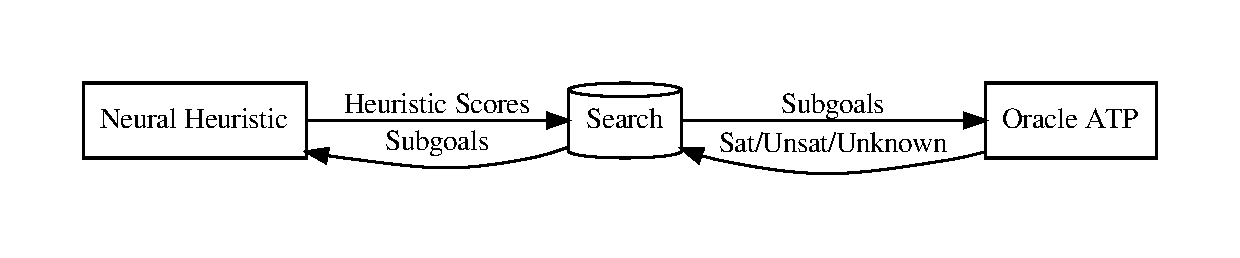
\includegraphics[width=0.8\textwidth]{architecture}
	\caption{A cartoon showing information flow in the proposed system.}
\end{figure}

\subsection{Publications}
The work on dynamic heuristic scheduling yielded a conference talk at AITP 2018~\cite{AITP}, and will also be presented and published at the PAAR 2018 workshop this summer.
I also presented initial findings for a currently-abandoned research direction at ARW 2018~\cite{ARW}.

\subsection{Thesis Sections}
Since I now have a reasonable grasp of previous work in this area, and some published material, the introductory and background thesis sections could be completed, along with a content section discussing the work on heuristic scheduling.

\section{Planning}
\subsection{Research Timetable}
Looking forward, I plan to finish the prototype of the distributed prover as soon as possible, at least by the start of the next year.
From there, a number of promising research directions appear, of which I can explore any number of the most promising:
\begin{itemize}
	\item Further machine-learning techniques and research for a better heuristic function.
	\item Engineering for efficiency.
	\item Engineering for arbitrary scaling.
	\item Different proof calculi: which works best for heuristic search?
	\item More powerful (or arbitrary) logics.
	\item Integration with existing provers and counter-model generators.
	\item Application to novel domains
\end{itemize}
Any of these directions may be backed up with a suitable benchmark.
I plan to explore these directions for the majority of the coming year, hopefully producing significant results that can be published in higher-impact venues than those this year, such as CADE or IJCAI.
This leaves the last year for exploring any remaining avenues and writing/compiling/submitting a thesis, with some considerable time left as a buffer which will be filled with further research if no issues arise.

\subsection{Planned Thesis Sections}
The approximate chapter layout of my thesis will be the following, with a brief side-step into indirect proof guidance with heuristic scheduling, followed by the main body of the work:
\begin{enumerate}
	\item Introduction
	\item Background and Previous Work
	\item Aside: Experiments with Heuristic Scheduling
	\begin{enumerate}
		\item Methodology and Engineering
		\item Experiment
		\item Results
		\item Conclusions
	\end{enumerate}
	\item Representing Proof State in Neural Networks
	\begin{enumerate}
		\item Methodology
		\item Experiments
		\item Results
		\item Conclusions
		\item Other Applications
	\end{enumerate}
	\item A ``Smart'' Theorem Prover
	\begin{enumerate}
		\item Engineering
		\item Variations (potentially more than one sub-section)
		\item Benchmarks
		\item Comparison and Conclusions
	\end{enumerate}
	\item Overall Conclusions
\end{enumerate}

\subsection{Risk Management}
The main risk to complete is the case in which my current design for distributed heuristic theorem proving is unworkable, and all attempts to fix it fail.
I consider this unlikely, but there are several ``escape routes'' in the event of this happening.
\begin{itemize}
	\item Further work on heuristic scheduling: there is plenty still left to research here.
	\item Integrate research on proof state representation into clause selection in Vampire: this is a prover that is known to work, so presumably less likely to fail.
	\item Scale down the scope of the project such that I can still show that heuristic proof search is possible, if slow. This still has applications in domains such as mathematics.
\end{itemize}

I therefore think it is improbable that I fail to submit a thesis of some form.

\section{Conclusion}
I have a good understanding of existing material in my target area (namely application of machine learning to automated theorem provers), some existing conference and publication acceptances, promising ongoing research, and future plans with a view towards completion of a thesis.
Therefore, I believe I have a good case for progression.


\printbibliography
\end{document}
